\documentclass[11pt]{article}
\usepackage{mathtools}
\usepackage{mdframed}
\usepackage{fullpage}
\usepackage{amsfonts}
\usepackage{tikz}
\usepackage{fancyhdr}
\usepackage{lastpage}
\usepackage{graphicx}


%edit this for each class
\newcommand\name{John Collin Vincent}
\newcommand\classname{Com S 311}
\newcommand\assignment{Project 2 Report}


\newcounter{excounter}
\setcounter{excounter}{1}
\newcommand\ques[2]{\vskip 1em  \noindent\textbf{\arabic{excounter}\addtocounter{excounter}{1}.} \emph{#1} \noindent#2}
\newenvironment{question}{\ques{}\begin{quote}}{\end{quote}}
\newenvironment{subquestion}[1]{#1) \begin{quote}}{\end{quote}}

\pagestyle{fancy}
\rfoot{\name, page \thepage/\pageref{LastPage}}
\cfoot{}
\rhead{}
\lhead{}
\renewcommand{\headrulewidth}{0pt}
\renewcommand{\footrulewidth}{0pt}
\DeclarePairedDelimiter\ceil{\lceil}{\rceil}
\DeclarePairedDelimiter\floor{\lfloor}{\rfloor}


\begin{document}


  {\bf \classname \hspace{1cm} \assignment\hfill \name}
  \vskip 2em


  \begin{question}
    When crawling the internet I use a hashset to store the visited but invalid pages, and a HashMap to store the validated pages. I use a ArrayDeque to
    store the pages/edges yet to be validated. The reason i use a hashset for the invalid pages is i just need a quick way to check if a page has been
    determained as invalid already and the constant time access of a hashset is perfect for this. I use the HashMap to store the valid pages because
    that allows me to map the string for the page to a graph node which will store the edges as well. These two combined makes the visited set
    in the assignment description. I use The ArrayDeque because it has constant time add and pop methods and it follows the first in first out
    pattern which is perfect for my needs.\\\\
    For the BFS in the GraphProccessor I use a HashMap for the visited list because it allows me to map a visited node to the node that first visited it.
    This allows me to get the direct path from u to v by using getting the string, i, that v maps to and then the string that i maps to and so on until I
    get back to u. Again it has constant time add and access which are the two operations I use. I use a ArrayDeque for $Q$ because it has constant
    time add and pop.
  \end{question}

  \begin{question}
    WikiCS.txt when run with /wiki/Computer\_Science, max of 200, and topics as an empty set has a Vertex set size of 200, and an Edge set size of 2867
  \end{question}

  \begin{question}
    I have a screenshot of the terminal output for when I ran the GraphProcessor functions\\
    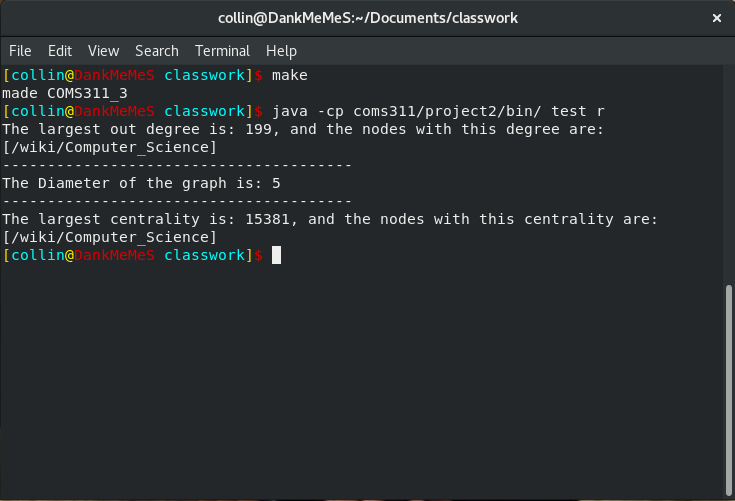
\includegraphics[width=6in, trim={0 8cm 2cm 0}, clip]{coms311/project2/output}
  \end{question}
  \clearpage
  \begin{question}
    The outDegree function has constant run time because it accesses the graph Node in the HashMap with contstant time and then returns the size of
    the out edge arraylist which is a constant time operation as well.\\\\
    The bfsPath function starts by going through each edge of the starting vertex and then going through each edge of those vertices, and so on until
    v is found. Every data structure operation in this process has constant run time so the runtime of this BFS is just based on the vertices and edges
    it accesses. This of coarse has a worst case run time of $O(|V| + |E|)$ because every vertex and edge might need to be accessed in order to find
    the vertex v. After this it backtraces the path and inserts the vertices into an arraylist, since it gets the nodes in the path from the HashMap
    it has constant access and inserting the Nodes into the Arraylist has constant runtime as well. So the runtime of this part of the function is
    just $O(|P|)$ where $P$ is the set of nodes in the Path from $u$ to $v$. So the overall runtime is $O(|V| + |E| + |P|)$\\\\
    The diameter function loops through the vertices in the graph and uses the bfsPath function to find the shortes path between every vertex in the graph.
    So the runtime of this function is $O(|V|^2)$ which each runs a bfsPath which is $O(|V| + |E| + |P|)$ so the overall runtime is
    $O(|V|^2(|V| + |E| + |P|))$\\\\
    the centrality function is similar to the diameter function in that it runs in $O(|V|^2)$ but it runs 3 bfsPath functions to find if there is a
    path from $i$ to $j$ that is a minimal path that also runs through $v$, so the overall runtime is $O(3|V|^2(|V| + |E| + |P|))$
  \end{question}


\end{document}
